%%%%%%%%%%%%%%%%%%%%%%%%%%%%%%%%%%%%%%%%%
% University/School Laboratory Report
% LaTeX Template
% Version 3.1 (25/3/14)
%
% This template has been downloaded from:
% http://www.LaTeXTemplates.com
%
% Original author:
% Linux and Unix Users Group at Virginia Tech Wiki 
% (https://vtluug.org/wiki/Example_LaTeX_chem_lab_report)
%
% License:
% CC BY-NC-SA 3.0 (http://creativecommons.org/licenses/by-nc-sa/3.0/)
%
%%%%%%%%%%%%%%%%%%%%%%%%%%%%%%%%%%%%%%%%%

%----------------------------------------------------------------------------------------
%	PACKAGES AND DOCUMENT CONFIGURATIONS
%----------------------------------------------------------------------------------------

\documentclass[12pt]{article}

%\usepackage[version=3]{mhchem} % Package for chemical equation typesetting
%\usepackage{siunitx} % Provides the \SI{}{} and \si{} command for typesetting SI units
\usepackage[left=1in,top=1in,right=1in,bottom=1in]{geometry} % Document margins
\usepackage{graphicx} % Required for the inclusion of images
\usepackage{pdfpages}
\usepackage{natbib} % Required to change bibliography style to APA
\usepackage{amsmath} % Required for some math elements 

\setlength\parindent{0pt} % Removes all indentation from paragraphs

\renewcommand{\labelenumi}{\alph{enumi}.} % Make numbering in the enumerate environment by letter rather than number (e.g. section 6)

%\usepackage{times} % Uncomment to use the Times New Roman font

%----------------------------------------------------------------------------------------
%	DOCUMENT INFORMATION
%----------------------------------------------------------------------------------------

\title{\textbf{Find A Room} \\ Sprint 3 Planning Document \\ CS 307} % Title

\author{Team \textsc{13}(Snoxy)} % Author name

\date{\today} % Date for the report

\begin{document}

\maketitle % Insert the title, author and date

\begin{center}
\begin{tabular}{l r}
Members: & Nathan Chang \\ % Partner names
& Xiaojing Ji \\
& Zilun Mai(Owen) \\
& Saranyu Phusit(Gott, Team leader) \\
& Yao Xiao \\
\\
\bigskip
Instructor: & Professor Buster Dunsmore \\% Instructor/supervisor 
Project Coordinator: & Miguel Villarreal-Vasquez % Instructor/supervisor

\end{tabular}
\end{center}

% If you wish to include an abstract, uncomment the lines below
% \begin{abstract}
% Abstract text
% \end{abstract}

%----------------------------------------------------------------------------------------
%	SECTION 1
%----------------------------------------------------------------------------------------


\newpage

\section{Sprint Overview}

Navigating user to the destination.


\subsection{Scrum master}
\begin{itemize}
\item Saranyu Phusit, who has experience in developing mobile applications using tools similar to Phonegap.
\end{itemize}
\subsection{Meeting Schedule}
During the class time and during a day every weekend.


\section{Current Sprint Detail}

\subsection{Functional user story for this sprint}


\textbf{As a user...}
\begin{itemize}

\item I would like to see the suggestions while inputting the destination
\item I would like to see the shortest path to my destination highlighted on the map
\item I would like to have a step-by-step instructions to guide me to the destination
\item I would like be able to re-input my location if I am away from the directions.
\item I would like to be able to manipulate the map to view where I am better
\item I would like to have a good user experience using an app
\item I would like to be able to communicate with people who are currently inside the building.

\end{itemize}


\subsection{Task details}

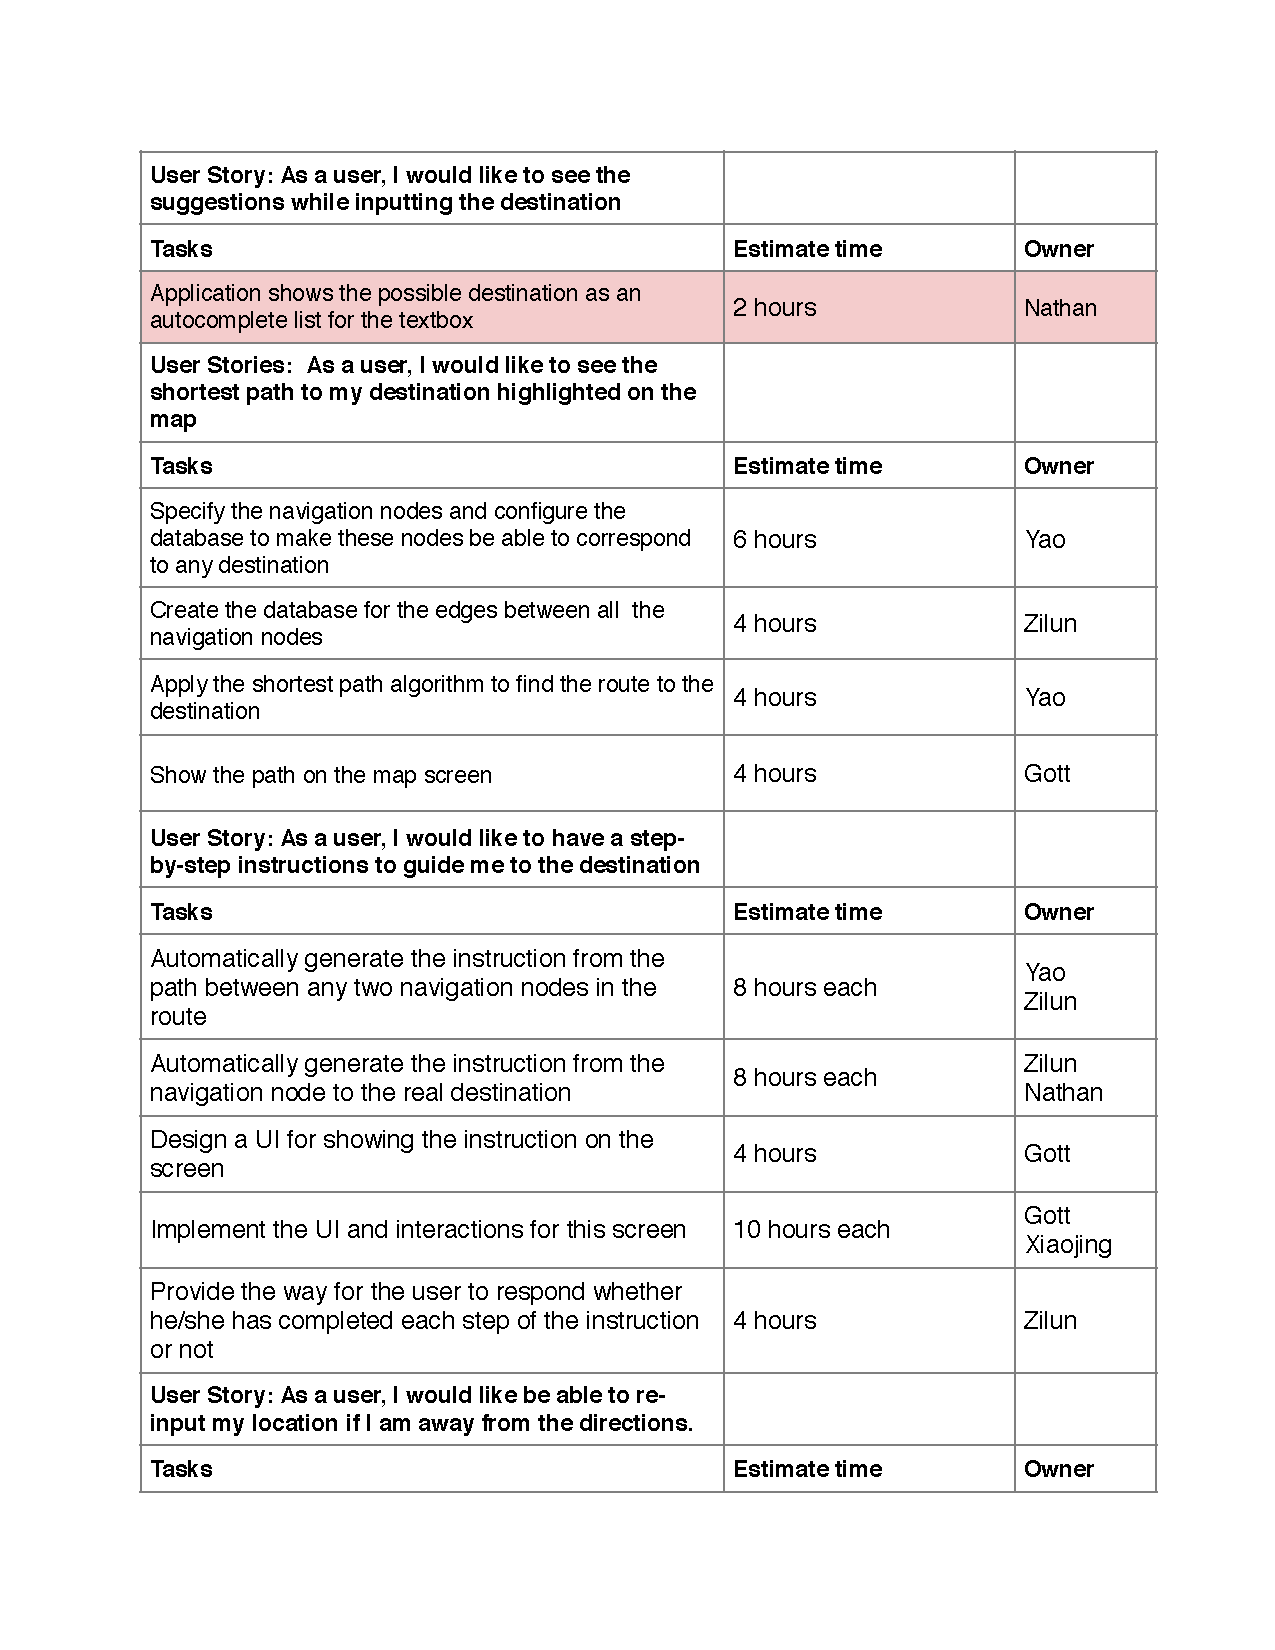
\includepdf[pages={1,2}]{tasks-details-sprint3.pdf}
%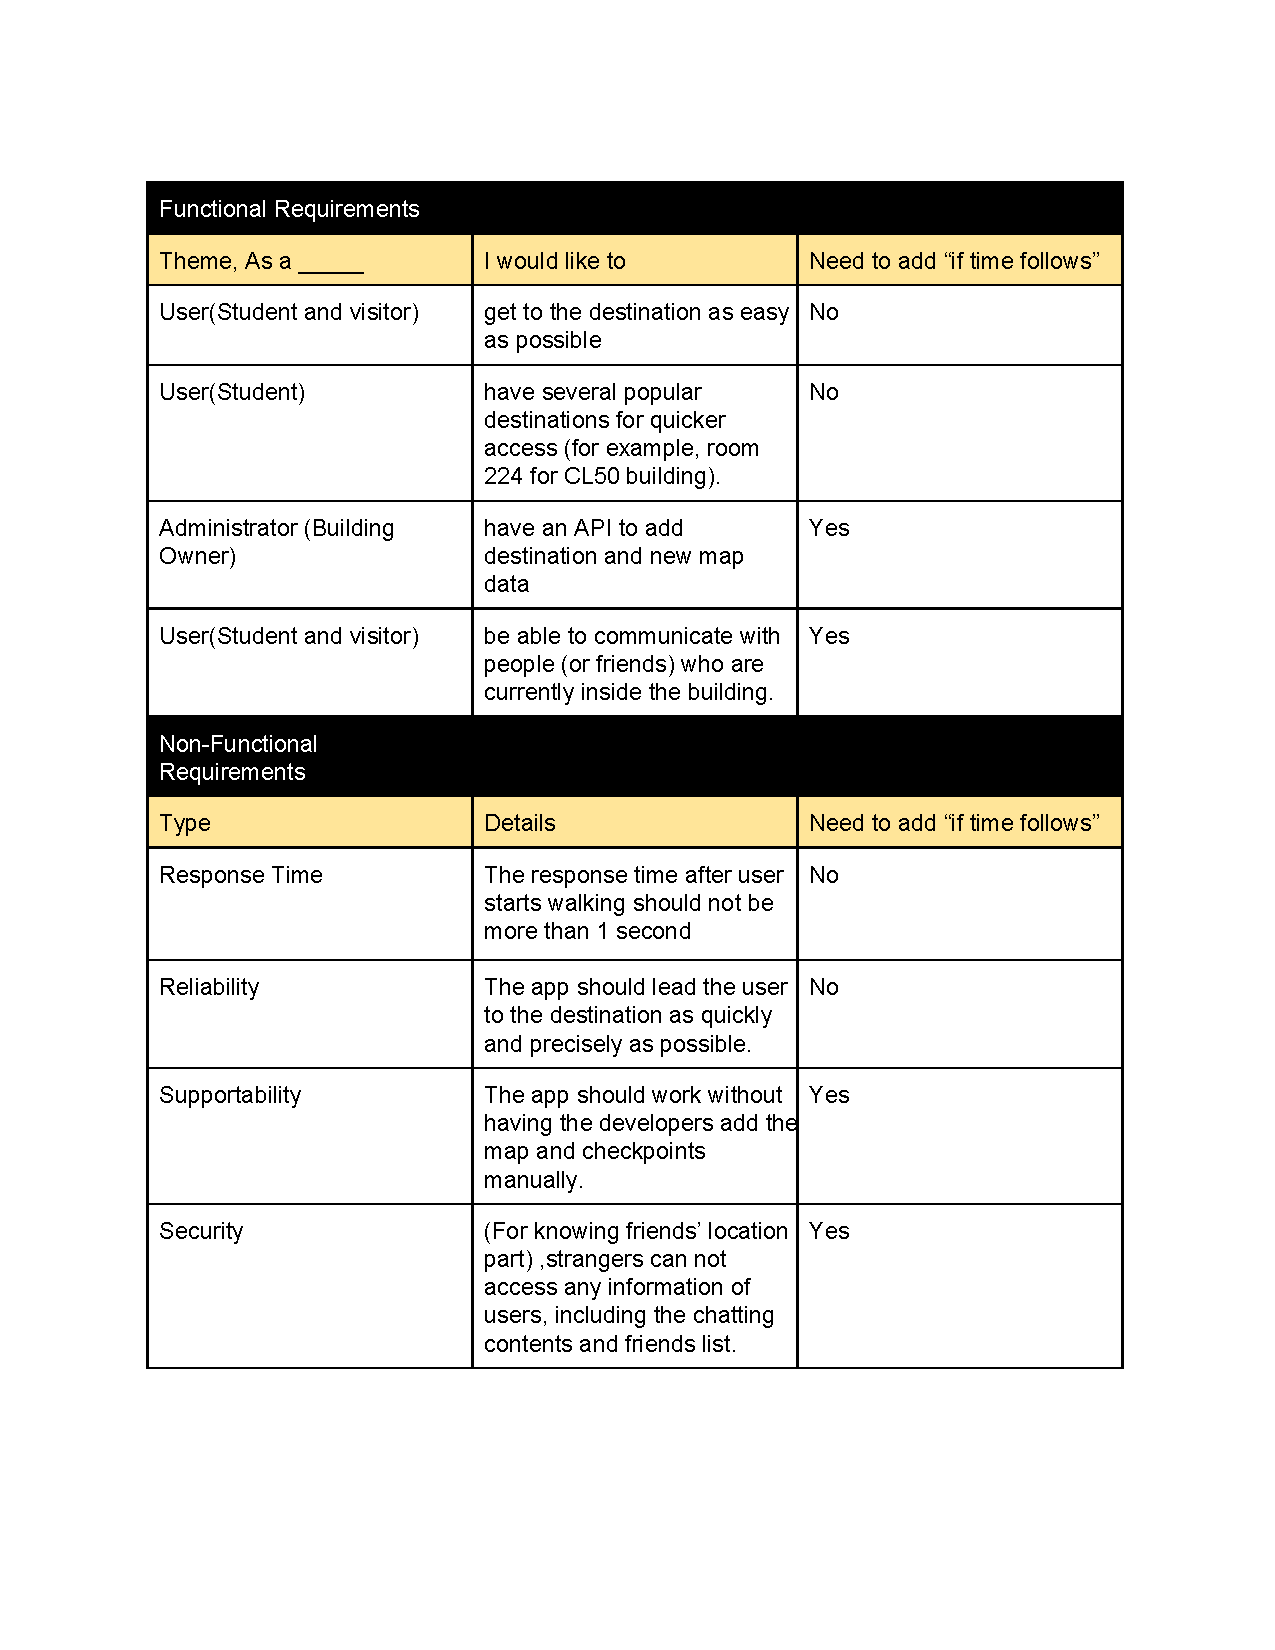
\includepdf{Sprint2Userstories.pdf}

The remaining user story:

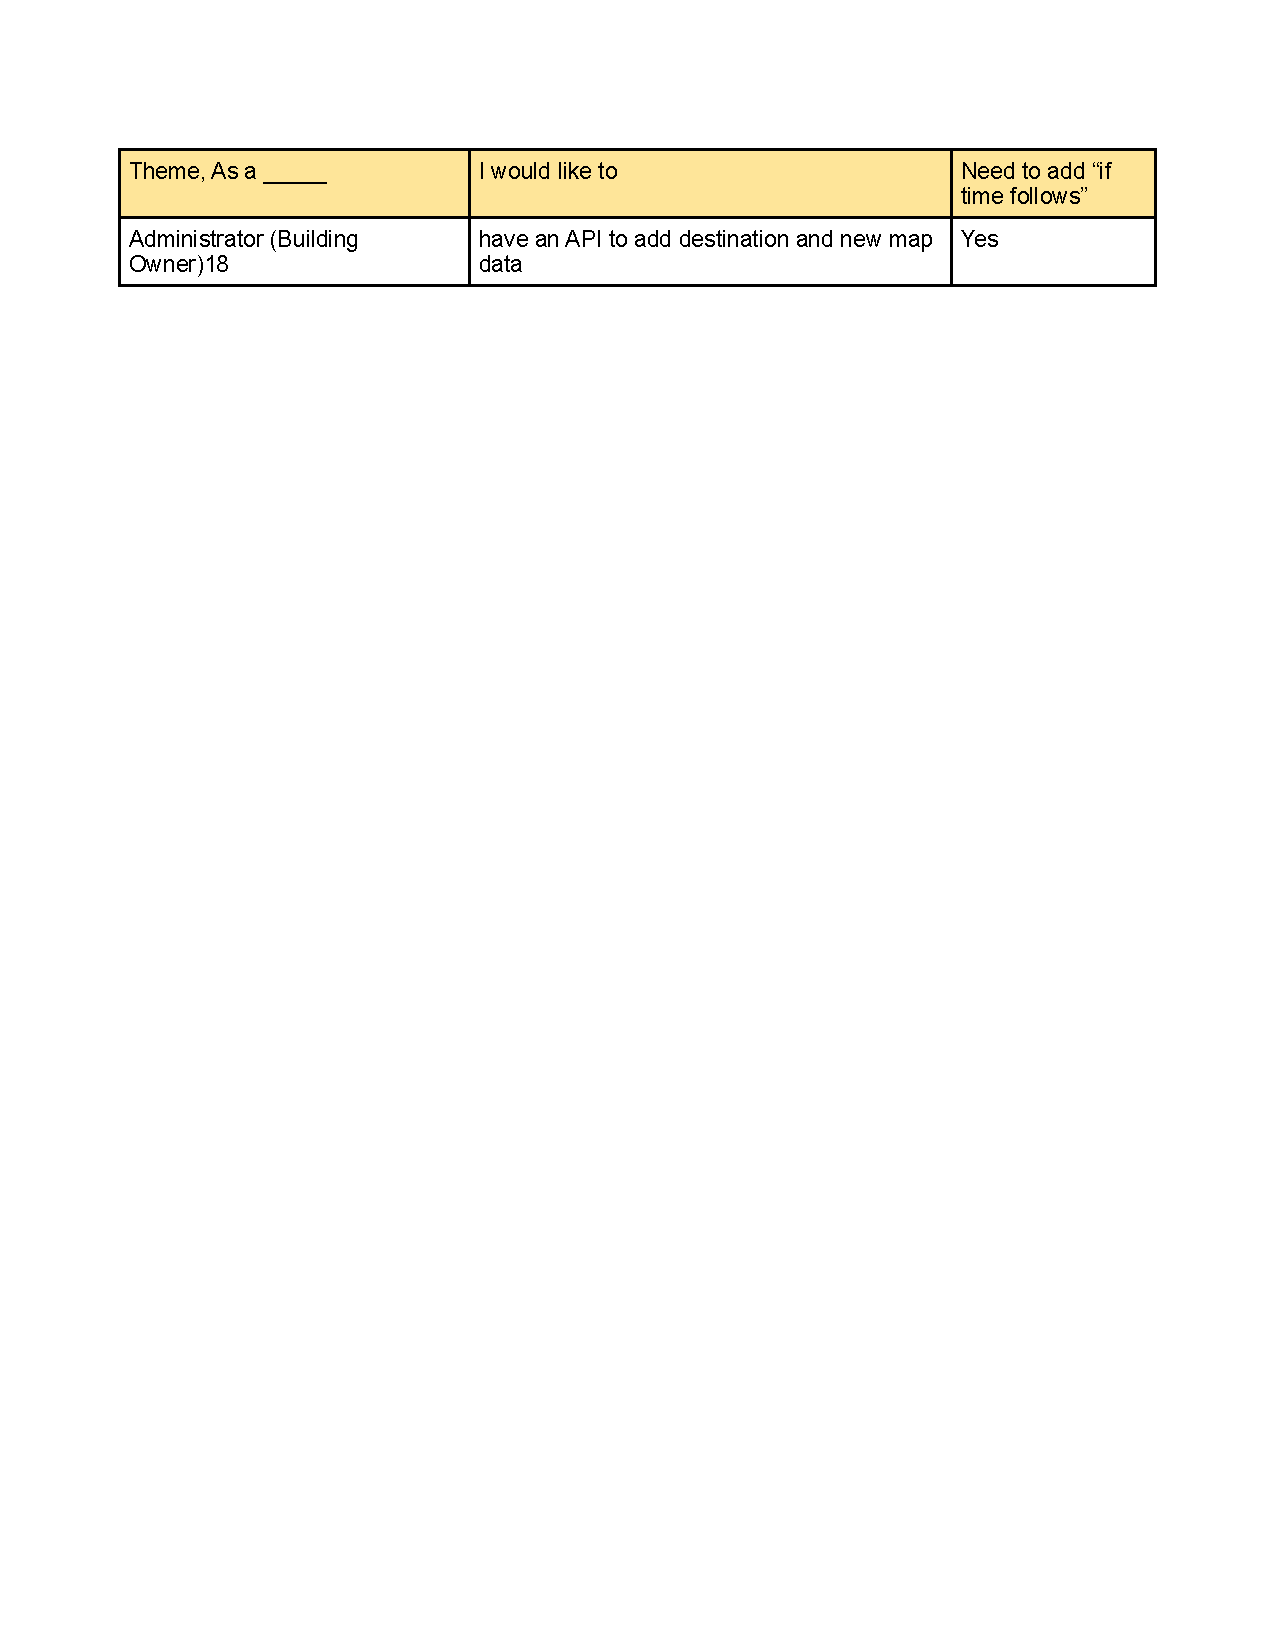
\includepdf[pages={1}]{remaining-user-story.pdf}


\end{document}